\subsection{Analisi}

\textbf{Periodo:} dal 2020-11-26 al 2021-01-14
\\ Le precondizioni sono:
\begin{itemize}
    \item Formazione del gruppo;
    \item Presentazione dei Capitolati.
\end{itemize}

Le postcondizioni sono:

\begin{itemize}
    \item Scelta del nome e del logo del gruppo;
    \item Creazione della mail e di una repository GitHub;
    \item Scelta del capitolato;
    \item Redazione dei documenti sopra descritti;
    \item Verifica e approvazione di quanto redatto.
\end{itemize}


Quest fase è composta da sette attività che corrispondono ai documenti prodotti:
\begin{itemize}
    \item \textbf{\textit{Studio di Fattibilità}}: Vengono analizzati i vari capitolati per evidenziare aspetti
negativi e positivi per trovare quello più adatto al gruppo. L'attività è bloccante per l'analisi dei requisiti;

    \item \textbf{\textit{Norme di Progetto}}: Vengono definite tutte le regole che il gruppo
\Gruppo dovrà seguire per la stesura dei documenti e per lo sviluppo del progetto;

    \item \textbf{\textit{Glossario}}: Contiene tutti i termini che possono risultare ambigui durante
lo svolgimento del progetto; di essi viene fornita una definizione sintetica ed esaustiva;

    \item \textbf{\textit{Lettera di Presentazione}}: Documento in cui il gruppo \Gruppo si candida al capitolato
scelto come fornitore del prodotto software richiesto;

    \item \textbf{\textit{Piano di Progetto}}: Il presente documento: in questo vengono descritte le attività,
i compiti e i rischi del progetto. Presenta poi la suddivisione del lavoro tra i membri del gruppo \Gruppo e il calcolo del preventivo;

    \item \textbf{\textit{Analisi dei Requisiti}}: Vengono studiati e analizzati nel dettaglio i requisiti del capitolato scelto nello \textit{Studio di Fattibilità};

    \item \textbf{\textit{Piano di Qualifica}}: Si individuano metodi e procedure per garantire la qualità del prodotto.
\end{itemize}

La pianificazione di questa fase è stata organizzata nelle seguenti sotto-fasi:

\begin{enumerate}
\item \textbf{2020-11-26 - 2020-12-10}:
    Inizio della stesura delle \NdP per avere delle regole condivise dal gruppo per svolgere il lavoro. Durate la stesura di queste il gruppo si confrontava riguardo ai vari capitolati rispetto ai loro aspetti positivi e negativi e all'esperienza che ogni componente aveva nel determinato ambito. Dopo gli iniziali confronti si è potuto iniziare uno \SdF generico per tutti i capitolati per poi approfondirlo per i capitolati che suscitavano più interesse al gruppo e iniziare a stilare il \textit{Glossario} per la registrazione dei termini, usati nei documenti, che potrebbero creare ambiguità. Durante questo periodo sono state prese decisioni tecniche e logistiche quali: nome del gruppo, logo, indirizzo mail, creazione repository e i vari mezzi di comunicazione;
\item \textbf{2020-12-10 - 2020-12-22}:
    Inizio della stesura del \PdP, contenente la pianificazione del lavoro da svolgere e la suddivisione dei ruoli tra i membri del gruppo.
    Stesa una prima bozza della \textit{Lettera di Presentazione}, il cui completamento sarà fatto dopo la conclusione \PdP con lÔÇÖaggiunta del prospetto economico finale. Integrato il \Glossario quando necessario.
    Il 2020-12-22 Il gruppo ha fissato una milestone per il completamento dei documenti iniziati in queste prime fasi, ad eccezione dell'ultima sezione del \PdP destinata al consuntivo finale della fase successiva. Iniziano le attività di verifica incrementale per i documenti in corso di stesura;
\item \textbf{2020-12-22 - 2021-01-12}:
    Inizio della stesura dell'\AdR e del \PdQ, con l'esposizione dei criteri di valutazione della qualità scelti dal gruppo e le rispettive metriche di calcolo. Continuano le attività di verifica incrementale per i documenti in corso di stesura;
\item \textbf{2021-01-12 - 2021-01-14}
    Il gruppo svolge le attività di verifica sugli ultimi documenti, completa il \Glossario e uniforma tutti i prodotti alle regole stabilite nelle \NdP se necessario.
\end{enumerate}

\subsubsection{Diagramma di Gantt: Analisi}

\begin{figure}[ht]
    \centering
    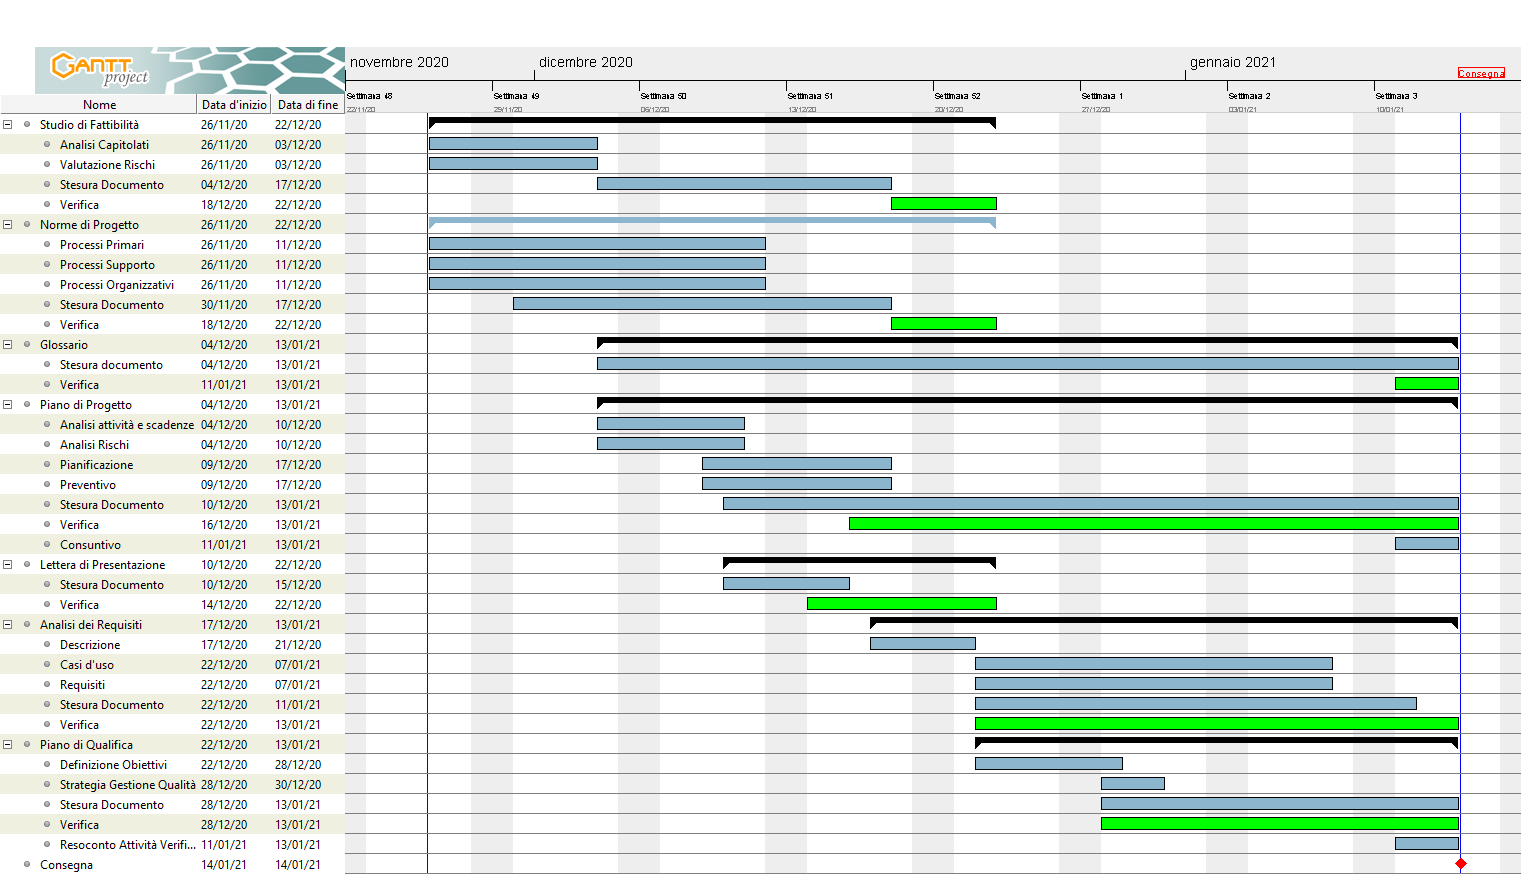
\includegraphics[width=\textwidth]{../../Immagini/Analisi}
    \caption{Diagramma di Gantt dell'avvitià di Analisi}
\end{figure}
